\documentclass{article}
\usepackage[utf8]{inputenc}
\usepackage{graphicx}

\title{Computational Physics (physics760)\\Exercise 2}
\author{Ajay S. Sakthivasan, Dongjin Suh}
\date{November 4, 2022}

\begin{document}

\maketitle

\section{Simulating the 2-D Ising Model}
In this homework, we implemented the \verb|Metropolis-Hastings| algorithm to simulate the 2D Ising Model. The calculation of total energy of a particular configuration is much more efficient in our implementation, due to the possibility of manipulating $numpy$ arrays. Figure \ref{fig:energy-calc} shows the evaluation times for arbitrary configurations with $N = 1, 2, ..., 20$, timed using \verb|timeit| on \verb|Python|. We see that the evaluation time grows only very weakly with $N$. This is due to the efficiency of $numpy$ manipulations.\\
\begin{figure}[h!]
    \centering
    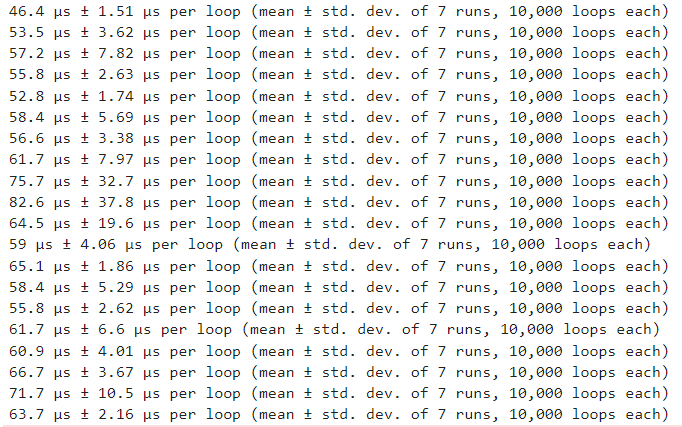
\includegraphics[width=.9\textwidth]{energy-calc.png}
    \caption{Evaluation time for arbitrary configurations with $N = 1, 2, ..., 20$}
    \label{fig:energy-calc}
\end{figure}
Similarly, calculations of energy before and after a spin flip shows a similar trend, as can be seen from the code. However, this step is implemented inside a $for-loop$, which makes it grow roughly quadratically with the number of lattice points. This step is at the heart of the \verb|Metropolis-Hastings| algorithm.\\
The critical coupling, $J_c$, gives the value of the coupling beyond which spontaneous magnetisation takes place for a given non-zero external magnetic field. This is an example of a phase transition, whose universality across different physical systems has been well studied. This can be seen from figure \ref{fig:mag-int-analy}. The value of $J_c$ is about $0.44$. Figure \ref{fig:energy-int-analy} shows the analytical result for energy vs. coupling factor.\\
\begin{figure}[h!]
    \centering
    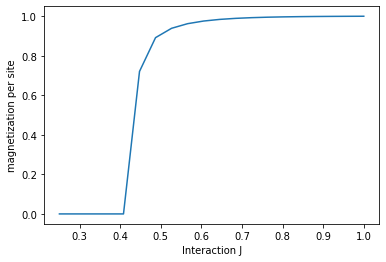
\includegraphics[width=.6\textwidth]{mag-int-analy.png}
    \caption{Analytical result for Magnetisation vs. Coupling factor}
    \label{fig:mag-int-analy}
\end{figure}
\begin{figure}[h!]
    \centering
    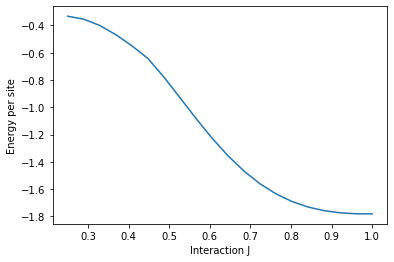
\includegraphics[width=.6\textwidth]{energy-int-analy.png}
    \caption{Analytical result for Energy vs. Coupling factor}
    \label{fig:energy-int-analy}
\end{figure} 

Figure \ref{fig:mag-h} shows magnetisation vs. external magnetic field for a fixed value of $J$. 
We can see as expected that the magnetization goes up from -1 to 1 by increasing the external field h. You can also see that the curve at field h = 0 passes through the zero magnetization, which was also to be expected. \\

\begin{figure}[h!]
    \centering
    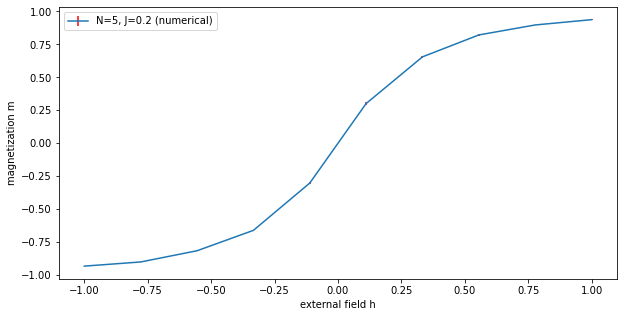
\includegraphics[width=.7\textwidth]{mag-h.png}
    \caption{Magnetisation vs. External field for a given coupling factor}
    \label{fig:mag-h}
\end{figure}

Figure \ref{fig:mag-int_N5} and \ref{fig:mag-int_N10} show the numerical result for magnetisation vs. coupling factor and figure \ref{fig:enrgy-int} shows the numerical result for energy vs. coupling factor. As can be seen, unfortunately we were unable to simulate the expected phase transitions in our numerical simulations. Especially the part, where we tried to simulate the energy against interaction J, does not show the phase transition very well. The only thing we could get from simulation is the continuous decreasing of energy by increasing J, but unfortunately it is not good to see how the energy drops steeply at the critical point of J and from J = 1 again shows a fairly flat curve, which is actually supposed to show the phase transition well.\\
We are actively trying to understand what went wrong with our simulations, and hopefully we are able to fix it in the near future. Our best guess at this point is that we are overlooking some trivial mistake in the implementation of the algorithm. \\
When simulating magnetization versus J, one can still see that magnetization begins to decrease rapidly for smaller J under the critical J. The magnetization should go directly to zero, as can be seen in the analytical solution. However, one can see that the curve for larger length of lattice N converges more and more towards zero when the interaction falls below the critical J = 0.44. \\

To the question what would happen if we plot $\langle m \rangle$, instead of $\langle \vert m \vert \rangle$, we would no longer observe any phase transition in that case.

\begin{figure}[h!]
    \centering
    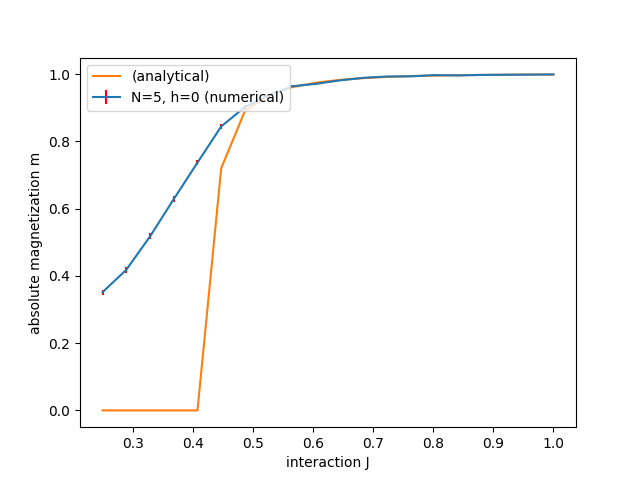
\includegraphics[width=.8\textwidth]{N5_numJ20.png}
    \caption{Magnetisation vs. Coupling factor for lattice size $N_{x,y}$ = 5 (Simulation)}
    \label{fig:mag-int_N5}
\end{figure}
\begin{figure}[h!]
    \centering
    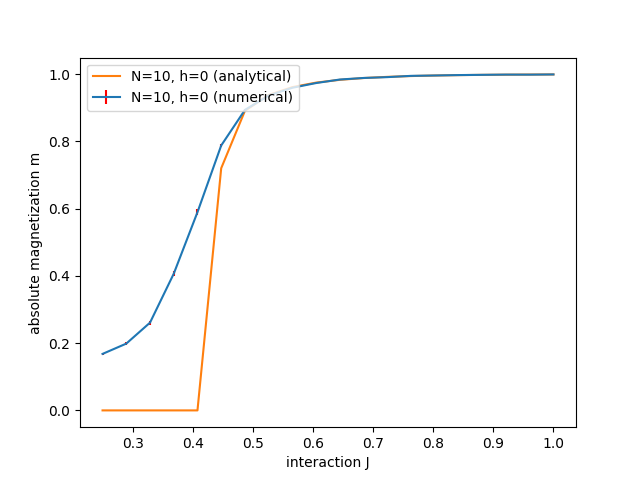
\includegraphics[width=.8\textwidth]{N10_numJ20.png}
    \caption{Magnetisation vs. Coupling factor for lattice size $N_{x,y}$ = 10  (Simulation)}
    \label{fig:mag-int_N10}
\end{figure}
\begin{figure}[h!]
    \centering
    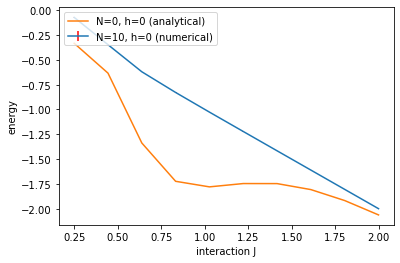
\includegraphics[width=.8\textwidth]{energy-int.png}
    \caption{Energy vs. Coupling factor (Simulation)}
    \label{fig:enrgy-int}
\end{figure}

\end{document}